\documentclass[tikz,border=10pt]{standalone}
\usepackage{tikz}
\usetikzlibrary{shapes,arrows,positioning,calc,fit,backgrounds}
\usepackage{amsmath}

\begin{document}

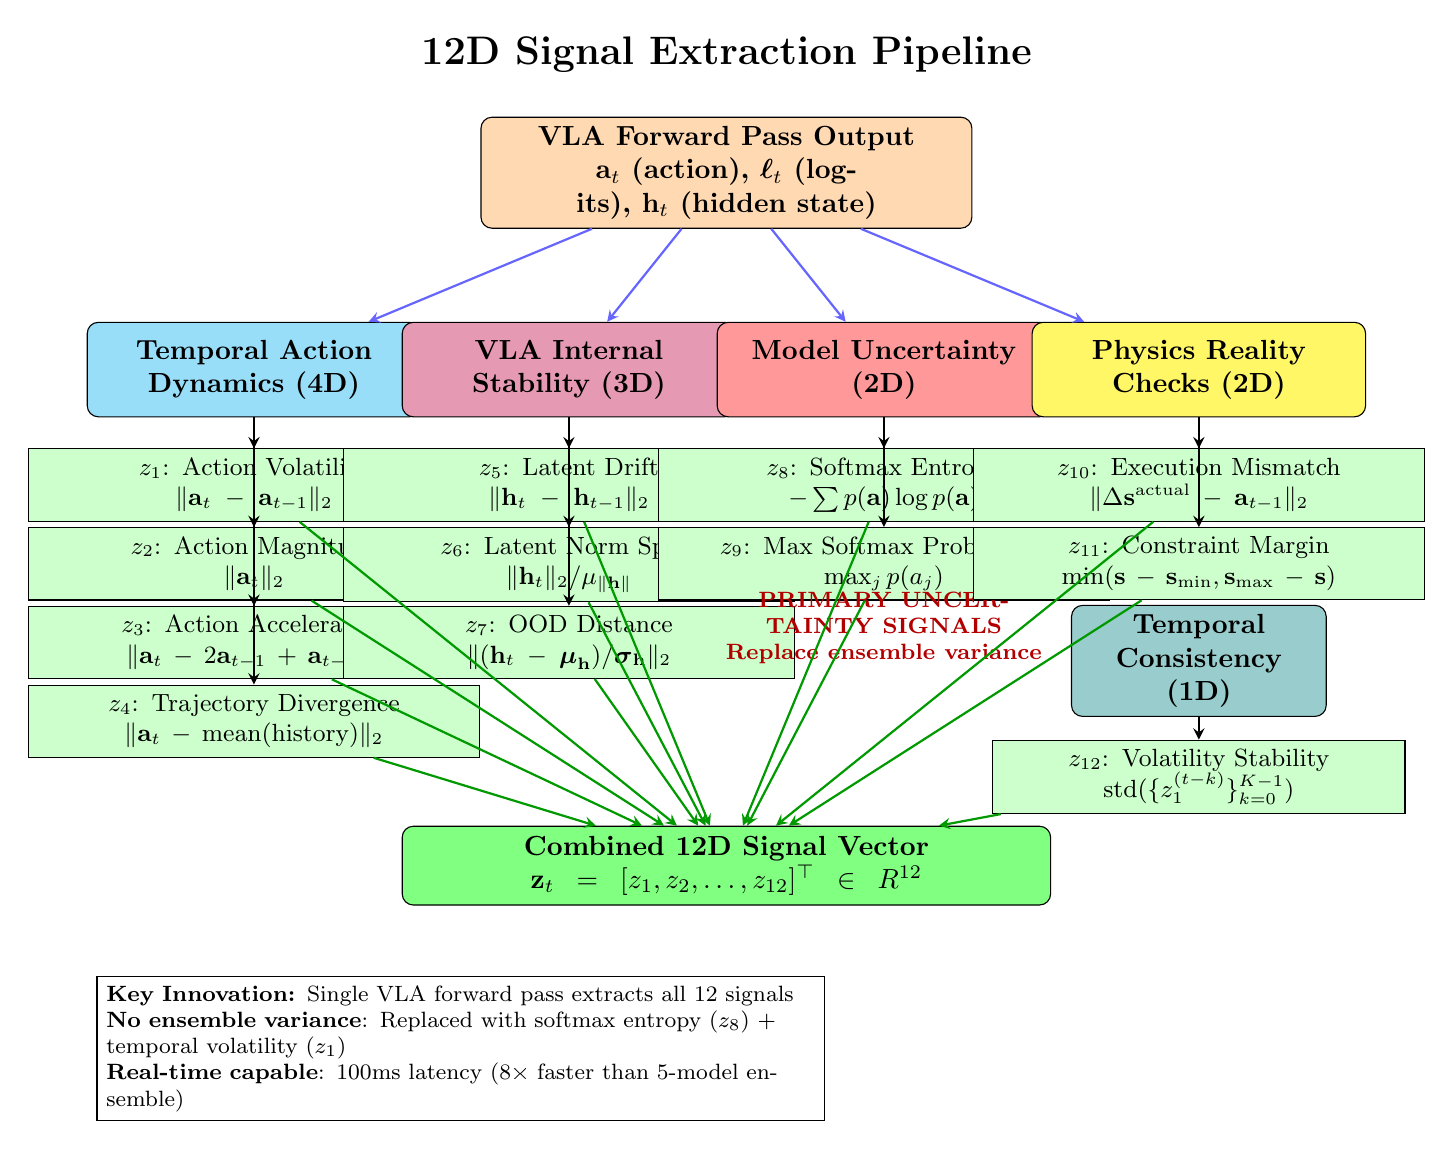
\begin{tikzpicture}[
    category/.style={rectangle, draw, fill=blue!30, text width=4cm, text centered, rounded corners, minimum height=1.2cm, font=\bfseries},
    signal/.style={rectangle, draw, fill=green!20, text width=5.5cm, text centered, minimum height=0.7cm, font=\small},
    equation/.style={text width=5cm, font=\footnotesize\ttfamily},
    arrow/.style={thick,->,>=stealth}
]

% Title
\node[font=\Large\bfseries] at (0, 8.5) {12D Signal Extraction Pipeline};

% VLA Output at top
\node[category, fill=orange!30, text width=6cm] (vla_output) at (0, 7) {
    VLA Forward Pass Output\\
    $\mathbf{a}_t$ (action), $\boldsymbol{\ell}_t$ (logits), $\mathbf{h}_t$ (hidden state)
};

% Category 1: Temporal Action Dynamics
\node[category, fill=cyan!40] (cat1) at (-6, 4.5) {Temporal Action\\Dynamics (4D)};

\node[signal, anchor=north] (sig1) at (-6, 3.5) {
    $z_1$: Action Volatility\\
    $\|\mathbf{a}_t - \mathbf{a}_{t-1}\|_2$
};

\node[signal, anchor=north] (sig2) at (-6, 2.5) {
    $z_2$: Action Magnitude\\
    $\|\mathbf{a}_t\|_2$
};

\node[signal, anchor=north] (sig3) at (-6, 1.5) {
    $z_3$: Action Acceleration\\
    $\|\mathbf{a}_t - 2\mathbf{a}_{t-1} + \mathbf{a}_{t-2}\|_2$
};

\node[signal, anchor=north] (sig4) at (-6, 0.5) {
    $z_4$: Trajectory Divergence\\
    $\|\mathbf{a}_t - \text{mean}(\text{history})\|_2$
};

% Category 2: VLA Internal Stability
\node[category, fill=purple!40] (cat2) at (-2, 4.5) {VLA Internal\\Stability (3D)};

\node[signal, anchor=north] (sig5) at (-2, 3.5) {
    $z_5$: Latent Drift\\
    $\|\mathbf{h}_t - \mathbf{h}_{t-1}\|_2$
};

\node[signal, anchor=north] (sig6) at (-2, 2.5) {
    $z_6$: Latent Norm Spike\\
    $\|\mathbf{h}_t\|_2 / \mu_{\|\mathbf{h}\|}$
};

\node[signal, anchor=north] (sig7) at (-2, 1.5) {
    $z_7$: OOD Distance\\
    $\|(\mathbf{h}_t - \boldsymbol{\mu}_\mathbf{h})/\boldsymbol{\sigma}_\mathbf{h}\|_2$
};

% Category 3: Model Uncertainty
\node[category, fill=red!40] (cat3) at (2, 4.5) {Model Uncertainty\\(2D)};

\node[signal, anchor=north] (sig8) at (2, 3.5) {
    $z_8$: Softmax Entropy\\
    $-\sum p(\mathbf{a}) \log p(\mathbf{a})$
};

\node[signal, anchor=north] (sig9) at (2, 2.5) {
    $z_9$: Max Softmax Probability\\
    $\max_j p(a_j)$
};

\node[font=\footnotesize\bfseries, text=red!70!black, text width=5cm, align=center, anchor=north] at (2, 1.8) {
    PRIMARY UNCERTAINTY SIGNALS\\
    Replace ensemble variance
};

% Category 4: Physics Reality Checks
\node[category, fill=yellow!60] (cat4) at (6, 4.5) {Physics Reality\\Checks (2D)};

\node[signal, anchor=north] (sig10) at (6, 3.5) {
    $z_{10}$: Execution Mismatch\\
    $\|\Delta\mathbf{s}^{\text{actual}} - \mathbf{a}_{t-1}\|_2$
};

\node[signal, anchor=north] (sig11) at (6, 2.5) {
    $z_{11}$: Constraint Margin\\
    $\min(\mathbf{s} - \mathbf{s}_{\min}, \mathbf{s}_{\max} - \mathbf{s})$
};

% Category 5: Temporal Consistency
\node[category, fill=teal!40, text width=3cm] (cat5) at (6, 0.8) {Temporal\\Consistency (1D)};

\node[signal, text width=5cm, anchor=north] (sig12) at (6, -0.2) {
    $z_{12}$: Volatility Stability\\
    $\text{std}(\{z_1^{(t-k)}\}_{k=0}^{K-1})$
};

% Final output
\node[category, fill=green!50, text width=8cm, minimum height=1cm] (output) at (0, -1.8) {
    Combined 12D Signal Vector\\
    $\mathbf{z}_t = [z_1, z_2, \ldots, z_{12}]^\top \in \mathbb{R}^{12}$
};

% Arrows from VLA output
\draw[arrow, blue!60, thick] (vla_output) -- (cat1);
\draw[arrow, blue!60, thick] (vla_output) -- (cat2);
\draw[arrow, blue!60, thick] (vla_output) -- (cat3);
\draw[arrow, blue!60, thick] (vla_output) -- (cat4);

% Arrows from categories to signals
\draw[arrow] (cat1) -- (sig1);
\draw[arrow] (cat1) -- (sig2);
\draw[arrow] (cat1) -- (sig3);
\draw[arrow] (cat1) -- (sig4);

\draw[arrow] (cat2) -- (sig5);
\draw[arrow] (cat2) -- (sig6);
\draw[arrow] (cat2) -- (sig7);

\draw[arrow] (cat3) -- (sig8);
\draw[arrow] (cat3) -- (sig9);

\draw[arrow] (cat4) -- (sig10);
\draw[arrow] (cat4) -- (sig11);

\draw[arrow] (cat5) -- (sig12);

% Arrows to final output
\draw[arrow, green!60!black, thick] (sig1) -- (output);
\draw[arrow, green!60!black, thick] (sig2) -- (output);
\draw[arrow, green!60!black, thick] (sig3) -- (output);
\draw[arrow, green!60!black, thick] (sig4) -- (output);
\draw[arrow, green!60!black, thick] (sig5) -- (output);
\draw[arrow, green!60!black, thick] (sig6) -- (output);
\draw[arrow, green!60!black, thick] (sig7) -- (output);
\draw[arrow, green!60!black, thick] (sig8) -- (output);
\draw[arrow, green!60!black, thick] (sig9) -- (output);
\draw[arrow, green!60!black, thick] (sig10) -- (output);
\draw[arrow, green!60!black, thick] (sig11) -- (output);
\draw[arrow, green!60!black, thick] (sig12) -- (output);

% Legend box
\node[draw, fill=white, text width=9cm, font=\footnotesize, align=left, anchor=north west] at (-8, -3.2) {
    \textbf{Key Innovation:} Single VLA forward pass extracts all 12 signals\\
    \textbf{No ensemble variance}: Replaced with softmax entropy ($z_8$) + temporal volatility ($z_1$)\\
    \textbf{Real-time capable}: 100ms latency (8× faster than 5-model ensemble)
};

\end{tikzpicture}

\end{document}
